\newpage
% 助教邮箱: denghaoran@zju.edu.cn
\section{AVL Trees, Splay Trees, and Amortized Analysis}

\subsection{AVL Trees}
\begin{itemize}
    \item [\textbf{Target}] Speed up searching (with insertion and deletion). 
    \item [\textbf{Tool}] Binary search trees. 
    \item [\textbf{Problem}] Although $T_p=O(height)$, but the height can be as bad as $O(N)$. 
\end{itemize}

\begin{definition}
    An empty binary tree is height balanced. If $T$ is a nonempty binary tree with $T_L$ and $T_R$ as its left and right subtrees, then $T$ is \hl{height balanced} iff 
    \begin{enumerate}
        \item $T_L$ and $T_R$ are height balanced, and 
        \item $|h_L -h_R|\le 1$ where $h_L$ and $h_R$ are the height of $T_L$ and $T_R$, respectively. 
    \end{enumerate}
\end{definition}
The empty tree height is -1. 

\begin{definition}
    The balance factor $BF(node)=h_L -h_R$. In an AVL tree, $BF(node)=-1,0,1$.
\end{definition}

\subsubsection{Tree rotation}
Tree rotation is an operation on a binary tree that changes the structure without interfering with the order of the elements. 

\begin{figure}[H]
    \centering
    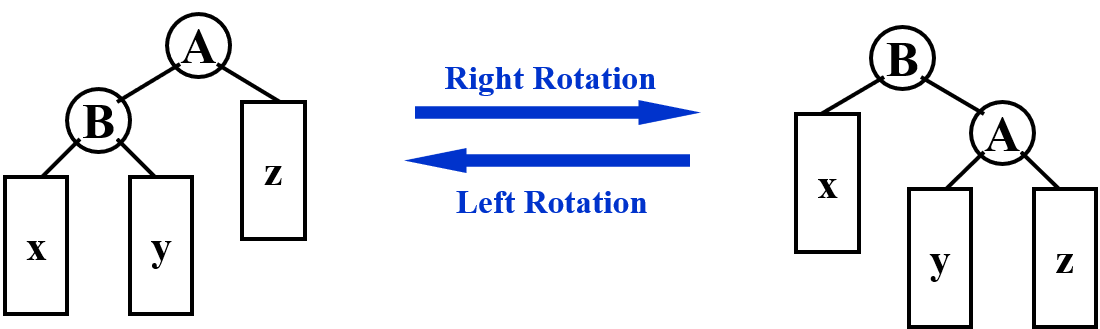
\includegraphics[width=0.309\textwidth]{ADS1/Tree rotation}
    \caption{Tree rotation}
\end{figure}

After a rotation, the side of the rotation increases its height by 1 whilst the side opposite the rotation decreases its height similarly. 

\begin{algorithm}[H]
    \caption{Right Rotation}
    \begin{algorithmic}
        \State tmp=B.rs
        \State B.rs=A
        \State A.ls=tmp
    \end{algorithmic}
\end{algorithm}

Time complexity: $O(1)$. 

(旋转的是平衡因子异常的结点)
\begin{enumerate}
    \item RR: the right subtrees's right subtree. 
    \begin{figure}[H]
        \centering
        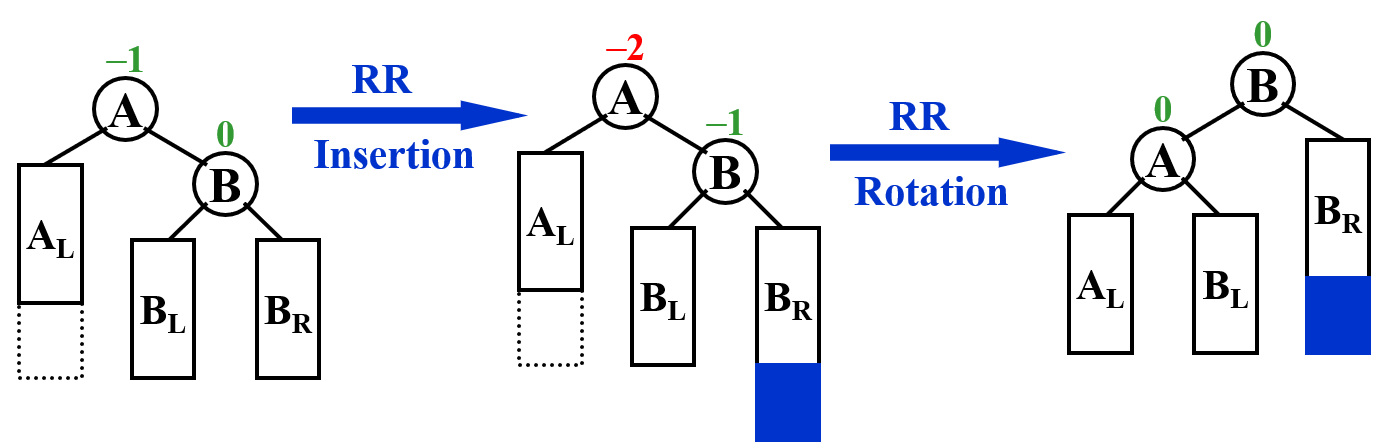
\includegraphics[width=0.309\textwidth]{ADS1/RR}
        \caption{RR}
    \end{figure}
    \item LL
    \begin{figure}[H]
        \centering
        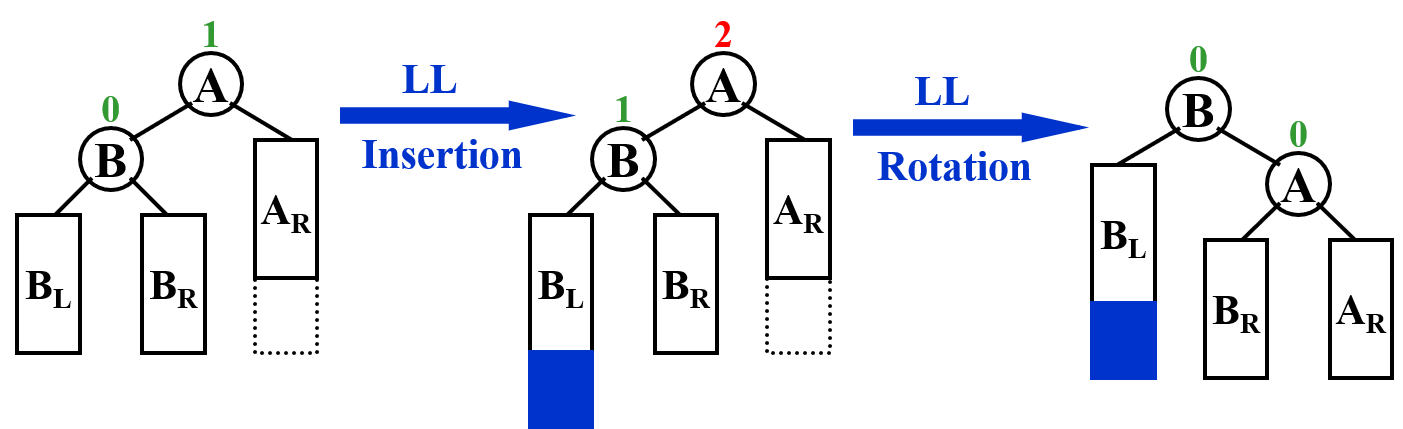
\includegraphics[width=0.309\textwidth]{ADS1/LL}
        \caption{LL}
    \end{figure}
    \item LR
    \begin{figure}[H]
        \centering
        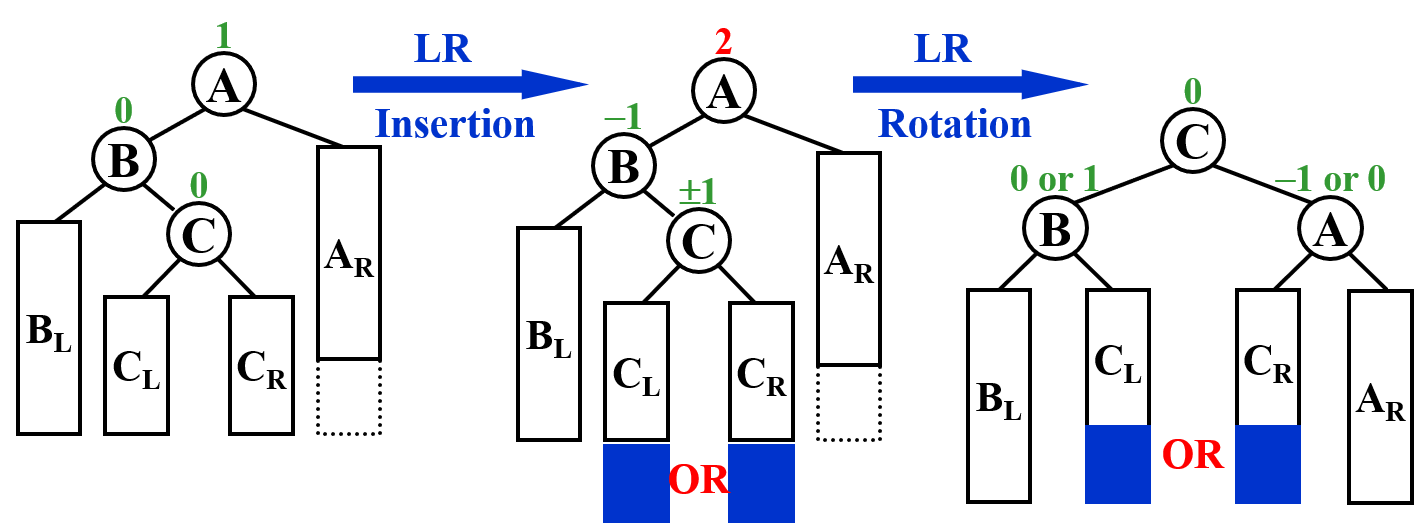
\includegraphics[width=0.309\textwidth]{ADS1/LR}
        \caption{LR}
    \end{figure}
    \item RL
    \begin{figure}[H]
        \centering
        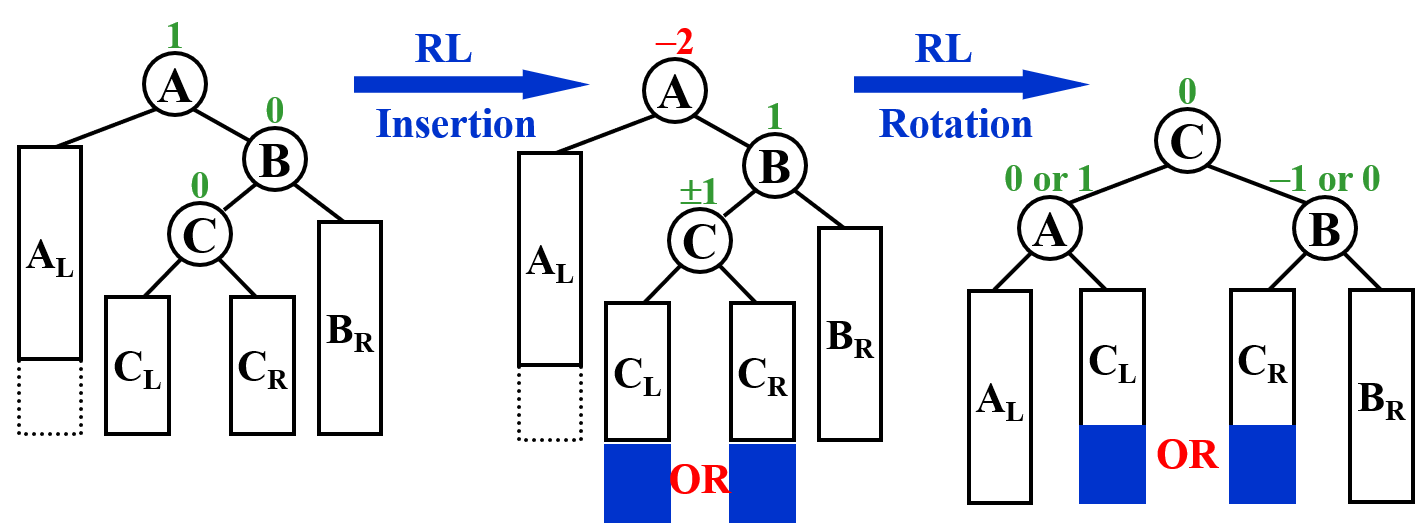
\includegraphics[width=0.309\textwidth]{ADS1/RL}
        \caption{RL}
    \end{figure}
\end{enumerate}

\subsubsection{Time Complexity of AVL}
Let $n_h$ be the minimum number of nodes in a height balanced tree of height $h$. Then the tree must look like 
\begin{figure}[H]
    \centering
    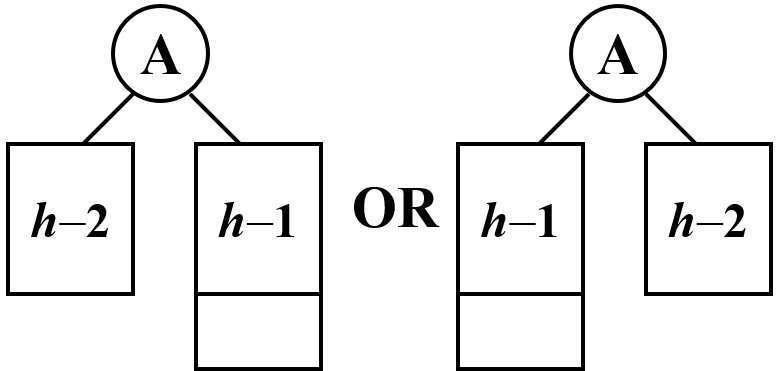
\includegraphics[width=0.209\textwidth]{ADS1/minimum AVL}
    \caption{minimum AVL}
\end{figure}
\begin{align*}
    n_h&=n_{h-1}+n_{h-2}+1\\
    \Rightarrow n_h&=F_{h+2}-1
\end{align*}
for $h\ge 0$. 
\begin{align*}
    F_i=&\frac{1}{\sqrt{5}}\left(\frac{1+\sqrt{5}}{2}\right)^i\\
    \therefore \, n_h\sim &a^{h+2}\\
    \therefore \, h=&O(\log n)
\end{align*}

\subsection{Splay Trees}

\begin{itemize}
    \item [\textbf{Target}] Any $M$ consecutive tree operations starting from an empty tree take at most $O(M\log N)$ time. 
\end{itemize}

It means taht the amortized time is $O(\log N)$. 

\subsubsection{Insertion}
For any nonroot node X, denote its parent by P and grandparent by G: 
\begin{enumerate}
    \item P is the root: Rotate X and P. 
    \item P is not the root:
    \begin{figure}[H]
        \centering
        \begin{minipage}{0.309\textwidth}
            \centering
            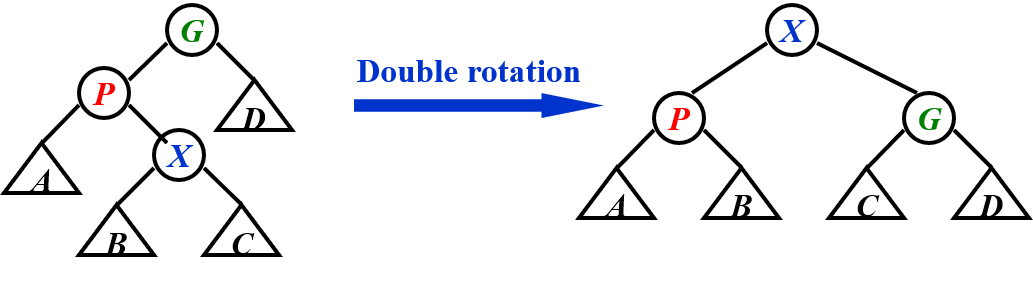
\includegraphics[width=\textwidth]{ADS1/zig-zag}
            \caption{zig-zag}
        \end{minipage}
        \begin{minipage}{0.309\textwidth}
            \centering
            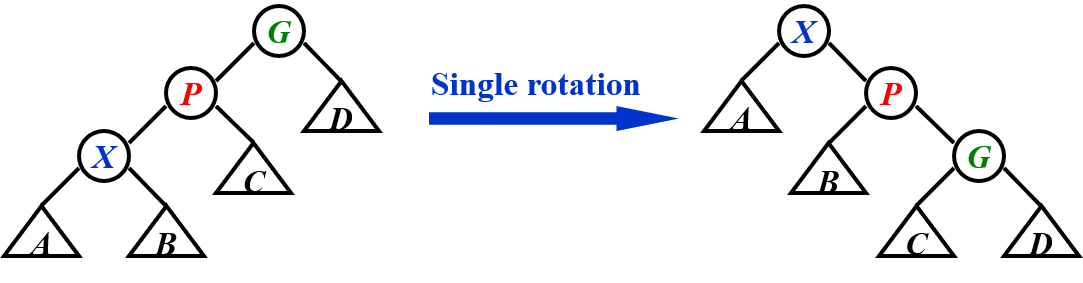
\includegraphics[width=\textwidth]{ADS1/zig-zig}
            \caption{zig-zig}
        \end{minipage}
    \end{figure}
\end{enumerate}

\subsubsection{Deletions}
\begin{enumerate}
    \item Find X. 
    \item Remove X. 
    \item Find Max ($T_L$) (X的前序结点). 
    \item Make $T_R$ the right child of the root of $T_L$. 
\end{enumerate}

\subsection{Amortized Analysis}
\begin{itemize}
    \item worst-case bound
    \item [$\ge$] amortized bound (Probability is not involved)
    \item [$\ge$] average-case bound
\end{itemize}

\subsubsection{Aggregate Analysis (聚合法)}
Show that for all $n$, a sequence of $n$ operations takes \hl{worst-case} time $T(n)$ in total. In the worst case, the average cost, or \hl{amortized cost}, per operation is therefore $\frac{T(n)}{n}$. 

\subsubsection{Accounting  method (合算法)}
When an operation's \hl{amortized cost} $\hat{c}_i$, exceeds its \hl{actual cost} $c_i$, we assign the difference to specific objects in the data structure as \hl{credit}. Credit can help pay for later operations whose amortized cost is less than their actual cost. 

Note: For all sequences of $n$ operations, we must have
\begin{align*}
    \sum_{i=1}^n\hat{c}_i\ge \sum_{i=1}^n c_i
\end{align*}

\subsubsection{Potential method (势能法)}

The credit 
\begin{align*}
    \hat{c}_i-c_i=Credit_i=\Phi(D_i)-\Phi(D_{i-1})
\end{align*}
$\Phi(D)$ is called potential function. $D$ represents the data structure. 

\begin{align*}
    \sum_{i=1}^n\hat{c}_i=&\sum_{i=1}^n \left(  c_i +\Phi(D_i)-\Phi(D_{i-1}) \right)\\
    =&\left(\sum_{i=1}^n c_i\right) + \Phi(D_n)-\Phi(D_0)
\end{align*}
$\Phi(D_n)-\Phi(D_0) \ge 0$. 

In general, a good potential function should always assume its minimum at the start of the sequence. 
 

%TODO 算法导论的摊还分析. 